\section{Theoretische Grundlagen}
    \subsection{Bandstruktur von Festkörpern}
        Zur Beschreibung der elektronischen Leiteigenschaften von Metallen wird meistens die Bandstruktur des Festkörpers genutzt. Diese stellt die Energiedispersion der Elektronen des Festkörpers dar, indem 
        die Bindungsenergie des Elektrons gegen dessen Impuls aufgetragen wird. Für Elektronen aus der s-Schale, die wie freie Elektronen betrachtet werden können, ergibt sich eine quadratische Abhängigkeit 
        der Energie vom Impuls und die Bänder sind parabolisch. Für stärker lokalisierte Elektronen, wie die aus der d-Schale, ergeben sich eher flache Bänder. Der Nutzen zur Charakterisierung von 
        Leitungseigenschaften wird erreicht, wenn die Fermi-Energie des Festkörpers mit in das Bandschema eingezeichnet wird, da das Verhalten der Bänder um die Fermi-Energie über die Leitfähigkeit
        entscheidet. Beim absoluten Nullpunkt der Temperatur sind alle Zustände über der Fermi-Energie unbesetzt und alle darunter besetzt. Sodass immer zwischen dem letzten vollständig besetzten Band, dem 
        Valenzband, und dem nächsthöheren, dem Leitungsband, unterschieden wird. Wenn die Fermi-Energie innerhalb des Leitungsbandes liegt, handelt es sich um ein Metall. Wenn die Fermi-Energie zwischen dem 
        Valenz- und Leitungsband liegt, entscheidet die Größe der Lücke über die Einordnung des Festkörpers. Liegt die Bandlücke in der Größenordnung einer Elektronenvolt handelt es sich um einen Halbleiter
        und wenn die Bandlücke größer ist um einen Isolator. Für Temperaturen über dem absoluten Nullpunkt kann nicht mehr so klar zwischen besetzten und unbesetzten Zuständen unterschieden werden, da die 
        Fermi-Dirac-Verteilung beginnt auszuschmieren und nun auch Zustände über der Fermi-Energie besetzt sein können. 

        \FloatBarrier

        \begin{figure}[h]
          \centering
          \includegraphics[width = 0.6\textwidth]{pictures/bandlücke.png}
          \caption{In der Abbildung sind die drei Unterscheidungen zur Kategorisierung von Festkörpern bezüglich ihrer Leitungsfähigkeit schematisch dargestellt. Entnommen aus \cite{demtroder_atome_2016}}
          \label{fig:Bandlücken}
        \end{figure}

        \FloatBarrier

    \subsection{Effektive Masse von Elektronen in Festkörpern}
        Zur Beschreibung von Teilchen ist es am besten, wenn diese möglichst frei sind, da dies einfache Bewegungsgleichungen mit sich zieht. Für Elektronen in Festkörpern ist dies leider nicht der Fall, weil
        sie durch das sie umgebende Kristallfeld ein Potential spüren, das abhängig von der Position im Gitter ist. Dies führt dazu, dass sie beim Wirken eines äußeren Feldes und der resultierenden Bewegung
        auch immer eine Potentialänderung erfahren. Um dennoch die grundlegenden Formeln bewegter Ladungen nutzen zu können, wird eine effektive Masse eingeführt, die die Potentialänderung bei Bewegung des
        Elektrons im Gitter berücksichtigt. Zur Einführung wird zunächst die Beschleunigung eines Elektrons im Festkörper als Ableitung der Gruppengeschwindigkeit nach der Zeit definiert
        
        \begin{equation*}
            \vec{\text{a}} = \frac{\text{dv}_{\text{g}}}{\text{dt}} = \frac{1}{\hbar} \cdot \left(\frac{\text{d}^2\text{E}}{\text{dk}^2}\right) \cdot \frac{\text{d}\vec{\text{k}}}{\text{dt}}
            \label{eqn:beschleunigung}
        \end{equation*}
        
        die porportional zur doppelten Ableitung der Energiedispersion nach dem Impuls und der Ableitung des Impulses nach der Zeit ist. Um die gewünschte Beschreibung des Kirstallelektrons als freies Elektron
        zu erreichen wird die Definition der Bewegungsgleichung nach der Ableitung des Impulses nach der Zeit umgestellt

        \begin{equation*}
            \vec{\text{F}} = \frac{\text{d}\vec{\text{p}}}{\text{dt}} = \hbar \frac{\text{d}\vec{\text{k}}}{\text{dt}} \qquad \longrightarrow \qquad  \frac{\text{d}\vec{\text{k}}}{\text{dt}} = \frac{\vec{\text{F}}}{\hbar}
            \label{eqn:F_freiesElektron}
        \end{equation*}

        und in \ref{eqn:beschleunigung} eingesetzt

        \begin{equation*}
            \vec{\text{a}}  = \frac{1}{\hbar^2} \cdot \left(\frac{\text{d}^2\text{E}}{\text{dk}^2}\right) \cdot \vec{\text{F}}
        \end{equation*}

        sodass letztendlich die Bewegungsgleichung eines freien Elektrons unter Zuhilfenahme der effektiven Masse, die der inversen Krümmung der Dispersionsrelation entspricht, erreicht wird:

        \begin{equation*}
            \vec{\text{a}} = \frac{\text{1}}{\text{m*}} \cdot \vec{\text{F}} \qquad \text{mit} \qquad \text{m*} = \hbar^2 \cdot \left(\frac{\text{d}^2\text{E}}{\text{dk}^2}\right)^{-1}
            \label{eqn:eff_masse}
        \end{equation*}


    \subsection{Dotierung von Halbleitern}
        Um die Leitfähigkeit von elementaren Halbleitern zu steigern, können sie dotiert werden. Bei diesem Prozess werden Fremdatome in sehr geringen Konzentration von $10^{-4}$ bis $10^{-8}$ in die Struktur
        des Elemtarhalbleiters eingefügt. Meist handelt es sich bei dem elementaren Halbleiter um ein 4-wertiges Atom, dass also mit 4 Elektronen anderer Atomen eine Bindung eingehen kann. 
        
            \subsubsection*{n-Dotierung}
             Sind die neu hinzugefügten Atome 5-wertig, führt dies dazu, dass ein Elektron des hinzugefügten Atoms nur sehr schwach gebunden ist und als Leitungselektron fungieren kann. Da so ein annähernd 
             freies Elektron hinzugeüft wird, heißen die 5-wertigen Störatome Donatoren und die dotierten Halbleiter n-dotiert. Die neuen Elektronen befinden sich in einem sogenannten Donatorzustand, der nahe 
             dem Leitungsband, aber unter der Fermi-Energie liegt, sodass sie auch durch geringe äoßere Energieeinwirkungen in das Leitungsband angehoben werden können.
            
             \FloatBarrier

             \begin{figure}[h]
                \centering
                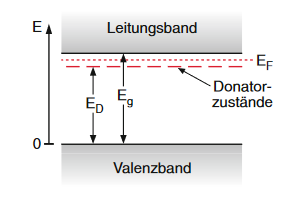
\includegraphics[width = 0.6\textwidth]{pictures/donator.png}
                \caption{Das zusätzliche freie Elektron befindet sich in einem Donatorzustand knapp unter der Fermi-Energie und nahe dem Leitungsband. Entnommen aus \cite{demtroder_atome_2016}}
                \label{fig:Donator}
             \end{figure}
     
             \FloatBarrier



            \subsubsection*{p-Dotierung}
            Werden stattdessen 3-wertige Atome eingebaut, fehlt ein Elektron zum eingehen der Bindung mit den elementaren Atomen. Dies erschafft einen Akzeptorzustand, der nahe dem Valenzband und über der 
            Fermi-Energie liegt. Dies ermöglicht Elektronen aus dem Leitungsband unter geringer Energieeinwirkungen über die Fermi-Energie gehoben zu werden und dabei zu leiten. Diese Art von Halbleitern wird 
            p-dotiert genannt.

            \FloatBarrier

            \begin{figure}[h]
                \centering
                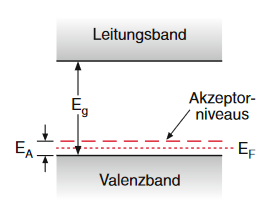
\includegraphics[width = 0.6\textwidth]{pictures/akzeptor.png}
                \caption{Durch das zur Bindung fehlende Elektron entsteht ein Akzeptorzustand nahe des Valenzbands und über der Fermi-Energie. Entnommen aus \cite{demtroder_atome_2016}}
                \label{fig:Akzeptor}
            \end{figure}
    
            \FloatBarrier


    \subsection{Zirkulare Doppelbrechung}
        Die zirkulare Doppelbrechung beschreibt die Drehung der Polarisationsebene von linear polarisertem Licht, wenn dieses ein optisch aktives Medium durchläuft. Zur Erklärung des Phänomens wird das linear 
        polariserte Licht in einen links-zirkulär und einen rechts zirkulär polarisierten Anteil aufgeteilt. Sobald dieses Licht in das optisch aktive Medium eintritt, erzeugt es eine Polarisation
        innerhalb des Materials

        \begin{equation}
            \vec{\text{P}} = \varepsilon_0 \cdot \underline{\underline{\chi}} \cdot \vec{\text{E}} 
            \label{eqn:polarisation}
        \end{equation}

        die von der Richtung des elektrischen Feldes des Lichts und des Suszeptibilität-Tensors $\underline{\underline{\chi}}$ des Materials abhängt. Dieser Tensor reduziert sich für isotope Medien zunächst
        auf ein Skalar. Bei nicht-isotropen Medien hingegen ergibt sich für $\underline{\underline{\chi}}$ eine Tensor 3. Stufe ergibt. Für diesen müssen zwei Fälle unterschieden werden. Wenn der Tensor 
        symmetrisch ist und alle Nebenachsenelemente durch DIagonalisieren eliminiert werden können, tritt kein Faraday-Effekt auf. Wenn der Tensor jedoch nicht verschwindende Nebenachsenelemente besitzt
        
        \begin{equation*}
            \underline{\underline{\chi}} =
            \begin{pmatrix}
                \chi_{\text{xx}} & \text{i} \chi_{\text{xy}} & 0 \\
                -\text{i}\chi_{\text{xy}} & \chi_{\text{xx}} & 0 \\
                0 & 0 & \chi_{\text{zz}}
            \end{pmatrix}
            \label{eqn:suszeptibilität}
        \end{equation*}

        lässt sich der Effekt der zirkularen Doppelbrechung erklären. Dazu wird das dielektrische Verschiebungsfeld $\vec{\text{D}} = \varepsilon_0 \cdot \vec{\text{E}} + \vec{\text{P}}$, welches für elektrische Felder
        innerhalb von Medien gilt, mit der nicht symmetrischen Suszeptibilität \ref{eqn:suszeptibilität} in die Wellengleichung von Licht eingesetzt

        \begin{equation*}
            \vec{\nabla} \times \left(\vec{\nabla} \times \vec{\text{E}}\right) = - \frac{1}{\text{c}^2} \cdot \left(1 + \underline{\underline{\chi}}\right) \cdot \frac{\partial^2\vec{\text{E}}}{\partial\text{t}^2}
        \end{equation*}

        in der die zeitliche Ableitung der Polarisation vernachlässigt wird, da das Material für gewöhnlich eine geringe Leitfähigkeit besitzt. Mit der Annahme einer sich in z-Richtung ausbreitenden 
        elektrischen Schwingung lässt sich die Wellengleichung nach Einsetzen der Suszeptibilität und des elektrischen Feldes in z-Richtung in die x-, y- und z-Komponente aufspalten. Die Gleichung für die 
        z-Komponente

        \begin{equation*}
            \frac{\omega^2}{\text{c}^2} \cdot \text{E}_{\text{z}} = \frac{\omega^2}{\text{c}^2} \chi_{\text{zz}} \cdot \text{E}_{\text{z}}    
        \end{equation*}

        zeigt, dass in dem gegebenen Fall die z-Komponente des elektischen Feldes verschwinden muss und die Welle sich somit transversal in z-Richtung ausbreitet. Die x- und y-Komponente ergeben ein 
        Gleichungssystem, das nur dann eine nicht-triviale Lösung besitzt, wenn die Determinante

        \begin{equation*}
            \left(-k^2 + \frac{\omega^2}{\text{c}^2} \cdot \left(1 + \chi_{\text{xx}}\right)\right)^2 - \left(\text{i} \cdot \frac{\omega^2}{\text{c}^2} \chi_{\text{xy}} \right)^2 = 0
        \end{equation*}

        verschwindet. Dies ist für zwei Wellenzahlen gegeben, die über die lineare Dispersionsrelation zwei mögliche Phasengeschwindigkeiten ergeben

        \begin{equation*}
            \text{v}_{\text{Ph}_{\text{R}}} = \frac{\text{c}}{\sqrt{1 + \chi_{\text{xx}} + \chi_{\text{xy}}}} \qquad \text{v}_{\text{Ph}_{\text{L}}} = \frac{\text{c}}{\sqrt{1 + \chi_{\text{xx}} - \chi_{\text{xy}}}}
            \label{eqn:Phasengeschwindigkeiten}
        \end{equation*}

        welche entweder für links- oder rechts-polarisertes Licht gelten. Aufgrund der unterschiedlichen Phasengeschwindigkeiten kommt es zur Drehung der Polarisation um den Winkel $\theta$

        \begin{equation*}
            \theta = \frac{\text{L}\omega}{2} \cdot \left(\frac{1}{ \text{v}_{\text{Ph}_{\text{R}}}} - \frac{1}{ \text{v}_{\text{Ph}_{\text{L}}}}\right)
        \end{equation*}

        die neben den Phasengeschwindigkeiten auch von der Länge des zurückgelegten Weges innerhalb des Mediums und der Frequenz des Lichts abhängt. Unter Zuhilfenahme einer Reihgenentwicklung bis zum linearen
        Term lässt sich der Rotationswinkel auch direkt von einer Suszeptibilitätskomponente ausdrücken.

        \begin{equation}
            \theta \approx \frac{\text{L}\omega}{2\text{cn}} \cdot \chi_{\text{xy}}
            \label{eqn:drehwinkel_näherung}
        \end{equation}


    \subsection{Faraday-Effekt}
        Der Faraday-Effekt beschreibt das Auftreten von zirkulare Doppelbrechung auch bei isotropen Medien, wenn ein äußeres Magnetfeld angelegt wird. Dies geschieht in Form der Rotation der Polarisationsebene
        des Lichts, das parallel oder anti-parallel zum magnetischen Feld verläuft. Zur Erklärung des Effekts muss zunächst die Bewegungsgleichung eines gebundenen Elektrons im  Einfluss äußerer Felder
        aufgestellt werden

        \begin{equation*}
            m \cdot \frac{\text{d}^2\vec{\text{r}}}{\text{dt}^2} + \text{K} \cdot \vec{\text{r}} = -\text{e} \cdot \vec{\text{E}}\text{(r)} - \text{e} \cdot \frac{\text{d}\vec{\text{r}}}{\text{dt}} \times \vec{\text{B}} \qquad \text{mit} \qquad \text{E(t)} \propto e^{-\text{i} \omega \text{t}}
        \end{equation*}

        wobei $\vec{\text{B}}$ das äußere B-Feld und $\vec{\text{E}}\text{(r)}$ das elektrische Feld des einfallenden Lichts beschreibt. Nach Ausrechnen der zeitlichen Ableitungen, Ersetzen des Ortsvektors
        $\vec{\text{r}}$ durch die Verschiebungspolarisation $\vec{\text{P}} = - \text{Ne} \vec{\text{r}}$ und Annahme eines Magnetfelds in z-Richtung ergeben sich die drei Komponenten der Bewegungsgleichungen.

        \begin{align*}
            \left(-\text{m}\omega^2 + \text{K}\right) \cdot \text{P}_{\text{x}} =& \text{Ne}^2 \cdot \text{E}_{\text{x}} + \text{ie} \omega \text{P}_{\text{y}} \text{B} \\
            \left(-\text{m}\omega^2 + \text{K}\right) \cdot \text{P}_{\text{y}} =& \text{Ne}^2 \cdot \text{E}_{\text{y}} - \text{ie} \omega \text{P}_{\text{y}} \text{B} \\
            \left(-\text{m}\omega^2 + \text{K}\right) \cdot \text{P}_{\text{z}} =& \text{Ne}^2 \cdot \text{E}_{\text{z}}
        \end{align*}

        Um den Drehwinkel zu bestimmen muss eine Komponente des Suszeptibilitättensors eingefügt werden, sodass die Polarisation über die, bereits im vorherigen Abschnitt definierte \ref{eqn:polarisation}, mit
        folgendem Ansatz 

        \begin{equation*}
            \underline{\underline{\chi}} =
            \begin{pmatrix}
                \chi_{\text{xx}} & \text{i} \chi_{\text{xy}} & 0 \\
                -\text{i}\chi_{\text{xy}} & \chi_{\text{xx}} & 0 \\
                0 & 0 & \chi_{\text{zz}}
            \end{pmatrix}
            \label{eqn:suszeptibilität}
        \end{equation*}

        für die Suszeptibilität ersetzt wird. Aus dem Gleichungssystem der 3 Komponenten geht hervor, dass die Suszeptibilität die selbe Form wie im Abschnitt zur zirkularen Doppelbrechung hat und somit auch 
        isotrope Medien bei Anlegen eines externen Magnetfelds doppelbrechend werden. Zudem lässt sich aus den Gleichungen ein Ausruck für die Komponente $\chi_{\text{xy}}$ finden, die eingesetzt in 
        \ref{eqn:drehwinkel_näherung} den Drehwinkel bestimmbar macht. Die zugehörige Gleichung

        \begin{equation*}
            \theta = \frac{\text{e}^3}{2\varepsilon_0\text{cm}^2} \cdot \frac{\omega^2}{\left(-\omega^2 + \frac{\text{K}}{\text{m}}\right)^2 - \left(\frac{\text{e}}{\text{m}} \cdot \text{B} \omega\right)^2} \cdot \frac{\text{NBL}}{\text{n}}
        \end{equation*}

        beinhaltet unter anderem den Term $\sqrt{\frac{\text{K}}{\text{m}}}$, der der Resonanzfrequenz $\omega_0$ der Elektronen im Medium entspricht und den Term $\frac{Be}{m}$, der der Zyklotronfrequenz 
        $\omega_{\text{c}}$ der Elektronen entspricht. N steht für die Dichte der Elektronen. Mit den Annahmen
        
        \begin{equation*}
            \left(\omega_0 - \omega\right)^2 >> \omega^2 \omega_{\text{C}}^2 \qquad \text{und} \qquad \omega << \omega_0
        \end{equation*}

        vereinfacht sich die Formel weiter und lässt sich durch die Wellenlänge des Lichts ausdrücken

        \begin{equation*}
            \theta(\lambda) \approx \frac{2\pi^2\text{e}^3\text{c}}{\varepsilon_0 \text{m}^2 \lambda^2 \omega_0^4} \cdot \frac{\text{NBL}}{\text{n}}
        \end{equation*}

        Für freie Elektronen verschwindet die rücktreibende Kraft und die Resonanzfrequenz geht gegen null. Dies führt zu einer weiterern Vereinfachung der Gleichung, erfordert aber auch das Ersetzen der Masse
        durch die effektive Masse, um weiterhin eine korrekte Beschreibung zu gewährleisten.

        \begin{equation}
            \theta_{\text{frei}}(\lambda) = \frac{\text{e}^3 \lambda^2}{8\pi^2\varepsilon_0 \text{c}^3} \cdot \frac{1}{\text{m*}} \cdot \frac{\text{NB}}{n}
        \end{equation}

        Dies erlaubt das Bestimmen der effektiven Masse über die Messung des Drehwinkels der Faraday-Rotation.



        